\documentclass[11pt]{exam}

\usepackage{listings}
\lstset{basicstyle=\footnotesize, showstringspaces=false,columns=fullflexible, basicstyle=\footnotesize\ttfamily, frame=tb }
\usepackage{pdfsync}
\usepackage{subfigure}
\usepackage{amsmath}
\usepackage{amsfonts}
\usepackage[pdftex]{graphicx}
\usepackage{enumitem}
\usepackage{fullpage}
\usepackage{wrapfig}
\usepackage[small]{caption}

\setlength{\parindent}{0in} % Removing indentation of new paragraphs

\title{Status Report}
\author{Mads Hartmann Jensen}

\begin{document}

\maketitle{}

\paragraph{} This report contains the details of my work for Hannes on his PhD project Kopitiam during my employment. The purpose is not to explain the theory behind the work but rather give an overview of what I've worked on and the state of completion as I leave the project. the My work includes build system setup and different kinds of static analysis of Java programs. \newline \newline

\newpage

\tableofcontents

\newpage

\section{Build System}

I switched the build system of the project to use the popular Scala
build tool SBT (Simple Build Tool) and set up support for automated
tests and automatic test coverage reports.

\newpage

\section{Live variable analysis}

\subsection{Motivation}

The scope of this analysis is to remove any superfluous temporary
variables introduced during the translation from Java to Simple Java
and as such it is not a normal dead variables analysis. \newline

It's a backwards analysis that traverses the program by blocks, so
when we're analyzing a block we know all of the variables that are
needed in the blocks of the rest of the program. It might help to think
of it as a liveliness analysis on a block-by-block basis rather than
statement-by-statement.\newline

If a variable is written in a block but not used in the rest of the
blocks then we might be able to remove the use of that variable. It's
not a dead variable in the usual sense because it might be used in
this block but because it's not used in the rest of the blocks we're
free to fiddle with it. There are a few exceptions to this that I will
cover later. \newline

An example would be this Simple Java Program. \newline

\begin{lstlisting}
class Fac {
  static int fac (int n) {
    int x;
    int tmp_1;
    if (n >= 0) {
      tmp_1 = this.fac(n - 1);
      x = n * tmp_1;
    } else {
      x = 1;
    };
    return x;
  }
}
\end{lstlisting}

In this case it would be much nicer if we could remove that temporary
variable tmp\_1 so we would have  \newline

\begin{lstlisting}
class Fac {
  static int fac (int n) {
    int x;

    if (n >= 0) {
      x = this.fac(n - 1);
      x = n * x;
    } else {
      x = 1;
    };
    return x;
  }
}
\end{lstlisting}

This is still a valid Simple Java program but it doesn't use the temporary
variable tmp\_1

\subsection{High Level Algorithm}

The analysis traverses the method body backwards by block. For each
block it calculates the set of variables that the block reads and
writes and uses this information to construct a set of variables that
are live at the beginning of the block. This information is then used
in the analysis of the previous block in the program. \newline

If a variable is written to in the current block but isn't in the live
set calculated from the next block then it means that the rest of the
method doesn't need the value we just wrote and it's only used in the
current block; i.e. we might be able to remove the use of that
temporary variable. In this case we attempt to rewrite the block, for
example, as shown in the previous example.. \newline

The analysis also covers two other special cases. The first occurs
when you read the same field of an object in each branch of an if-
statement. During the translation this will create a temporary
variable in each branch that represents the same object. In this case
we simply move the field read out of the if-statement and update the
branches to use that temporary variable. I realize now that this is
actually re-writing the original program and not only removing
superfluous temporary variable. The second occurs when the ternary
operator is used in assignments, see \texttt{src/test/resources/javaparser/Conditional3.txt}
for the example program that is used in the \texttt{OptimizerTest.scala} test.
Basically a simple program like the following:

\begin{figure}[h!]
\begin{lstlisting}
class Foo {
  int c;
  int b;
  void bar (int a) {
   b = a == c ? 20 : 30;
  }
}
\end{lstlisting}
\end{figure}

Results in the following Simple Java code:

\begin{figure}[h!]
\begin{lstlisting}
 class Foo {
   int c;
   int b;
   void bar (int a) {
    int tmp_2;
    Object tmp_1;

    tmp_2 = this.c;
    if (a == tmp_2) {
      tmp_1 = 20;
    } else {
      tmp_1 = 30;
    };
    this.b = tmp_1;
  }
}
\end{lstlisting}
\end{figure}

In this case we observe that the temporary variable that is being written to in both
branches of the if-statement is used in an assignment straight after. In this
case we simply move the assignment up into the if-statement branches like so:

\begin{figure}[h!]
\begin{lstlisting}
 void bar (int a) {
  int tmp_2;

  tmp_2 = this.c;
  if (a == tmp_2) {
    this.b = 20;
  } else {
    this.b = 30;
  };
}
\end{lstlisting}
\end{figure}

\subsection{Implementation}

The implementation can be found in the file
\texttt{src/main/scala/dk/itu/sdg/analysis/Optimizer.scala} and the tests
can be found in
\texttt{src/test/scala/dk/itu/sdg/analysis/OptimizerTest.scala}. \newline

You can run the analysis on a source file by typing the following in
an SBT session \texttt{run relative-path} and pick the main method
\texttt{dk.itu.sdg.javaparser.SimpleJavaOptimizedMain} which will
translate the Java file to Simple Java and optimize that. It will
print out the original Java program, the simple Java program and the
optimized simple Java program. \newline

\texttt{removeDeadVariables} is the main entry point which invokes
\texttt{liveVariableRewrite} which traverses the method body in
reverse order block by block. The analysis only traverses the body
once so the separation into blocks is done on the fly. This is done by
the internal \texttt{rec} method inside \texttt{liveVariableRewrite}.
It runs through the statements in the program in reverse order and
whenever it reads a statement that isn't  an instance of SJWhile or
SJConditional it simply adds the statement  to the current block and
continues backwards in the body of the method.  When there are no more
statements it finishes by analyzing the current  block. SJConditional
and SJWhile are considered block-separators, i.e. whenever one of
these statements are reached the current block accumulated so far is
analyzed and the block(s) of the SJConditional/SJWhile are processed.
The \texttt{rec} method is tail recursive and it keeps track of the
remaining statements (\texttt{List[SJStatement]}), the current block
(\texttt{List[SJStatement]}), the processed (i.e. result of rewrites)
lines so far (\texttt{List[SJStatement]}) and finally the set of
variables that are currently live (\texttt{HashSet[String]}). The re-
writing of normal blocks are taking care of by the method
\texttt{rewrite}. The  other two special cases are taken care of by
\texttt{removeSuperfluousInConditional}  and
\texttt{removeSuperfluousByTernary}. No mutable state is used in the implementation.


\subsection{State of Completion}

All the test cases pass. It might, however, be possible to find more
opportunities for optimization that I haven't thought of.

\newpage

\section{Purity analysis}

I've implemented a Purity analysis of Java programs based on the paper
A Combined Pointer and Purity Analysis for Java Program by Alexandru
Salcianu and Martin Rinard. I also presented the algorithm to the
Tools and Methods for Scalable Software Verification (TOMESO) group at
ITU.

\subsection{High Level Algorithm}

\subsubsection*{Data}

For each method a points-to graph is constructed; the points-to graph
consists of a set of nodes, a set of edges, the state of the local
variables and a set of globally escaped nodes. The \textbf{nodes}
model heap objects and can be of the following types:

\begin{itemize}
  \setlength{\itemsep}{1pt}
  \setlength{\parskip}{0pt}
  \item \emph{Inside Nodes} model the objects created by the analyzed method
  \item \emph{Outside Nodes} model the objects that are passed as arguments
        to the method
  \item \emph{Parameter Nodes} model the objects read from outside the method
\end{itemize}

The \textbf{edges} of the graph are used to model heap references. I will use
$<n1,f,n2>$ to denote an edge from n1 to n2, labeled with the field f;
intuitively, this edge models a reference from an object that n1
models to a node that n2 models, along field f. There are two kinds of
edges:

\begin{itemize}
  \setlength{\itemsep}{1pt}
  \setlength{\parskip}{0pt}
  \item \emph{Inside Edges} model the heap references created by the analyzed
        method
  \item \emph{Outside Edges} model the heap references read by the analyzed
        method from escaped objects. An object escapes if it is reachable
        from outside the analyzed method.
\end{itemize}

The \textbf{state of local variables} is represented using a
\texttt{Map[String, Set[Node]]}. For each method, the analysis also
computes a set of modified abstract fields. An \textbf{abstract field}
is a field of a specific node, i.e., a pair of the form $<n,f>$.

\begin{figure}[h!]
\begin{center}
  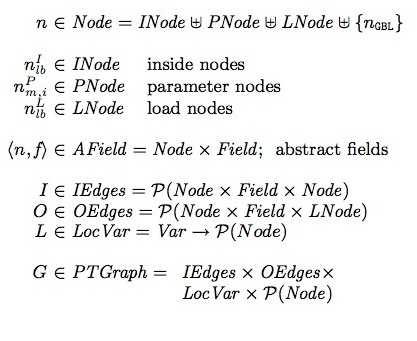
\includegraphics[width=0.5\textwidth]{data-representation}
\end{center}
\caption{Representaton of data as presented in the paper}
\label{data-notation}
\end{figure}

\subsubsection*{Algorithm}

As presented in the paper the algorithm consists of an intra- and
inter-procedural analysis. This separation, however, is largely
fictional as the inter-procedural analysis uses the intra-procedural
analysis and vice versa. Using this separation does make it easier to
explain the algorithm so I'll carry on in the same spirit. \newline

The \textbf{intra-procedural} analysis constructs a points-to graph of
a single method without knowing the calling context and  when a method
invocation occurs, say, when $m1$ invokes $m2$ then the \textbf{inter-
procedural} analysis instantiate the  parameterized result of $m2$ and
use that in the analysis of $m1$. \newline

The algorithm processes the strongly connected components of the call
graph from the leaves to the main method. Using a work-list it invokes
the  intra-procedural analysis on each method in the strongly
connected components until a fixed-point is reached. \newline

The intra-procedural analysis is a forward-flow analysis and for each
statement it uses a transfer function that given a points-to graph and
a statement will compute the points-to graph right after the
statement. It also computes the set of modified abstract fields. For a
detailed description of each of the transfer functions see the paper.
\newline

The inter-procedural analysis does four things:

\begin{itemize}
  \setlength{\itemsep}{1pt}
  \setlength{\parskip}{0pt}
  \item Constructs a node mapping from nodes of the points-to graph of
        $m2$ ($G_{callee}$) to nodes of the points-to graph of
        $m1$ ($G$). The node mapping disambiguates as many parameter-
        and load-nodes from the callee as possible
  \item Combines the graph $G$ and graph $G_{callee}$
  \item Simplifies the resulting graph
  \item Updates the set of modified abstract field
\end{itemize}

\subsubsection*{Using the results}

Once the analysis is done we have a points-to graph and a set of
abstract modified fields for each method in the program. We use these
to derive information abut the program. A \textbf{method is pure} if
the set of modified abstract fields is empty. If a method isn't pure
we can infer a regular expressions that describe all the pre-state
locations modified by $m$. This  is simply done by constructing a
finite state automaton $F$ with the following states:

\begin{itemize}
  \setlength{\itemsep}{1pt}
  \setlength{\parskip}{0pt}
  \item All the nodes from the points-to graph $G$
  \item An initial state s
  \item An accepting state t
\end{itemize}

And the following transitions:

\begin{itemize}
  \setlength{\itemsep}{1pt}
  \setlength{\parskip}{0pt}
  \item Each outside edge from $G$ generates a transition in $F$ labeled with
        the field of the outside edge
  \item For each parameter $p_i$ of $m$, we create a transition from $s$ to
        the corresponding parameter node, and label it with the parameter $p_i$
  \item For each mutated abstract field $<n,f>$ add a transition from $n$ to the
        accepting state $t$. Label it with the field $f$.
\end{itemize}

Now we can generate the regular expressions by recording the labels of
all paths from the start state to the accepting state.

\subsection{Implementation}

\subsubsection*{Source Files Overview}

The following files are all placed in the folder
\texttt{src/main/scala/dk/itu/sdg/analysis}

\begin{itemize}
  \setlength{\itemsep}{1pt}
  \setlength{\parskip}{0pt}
  \item The purity analysis algorithm can be found in \texttt{Purity.scala}
  \item The Strongly Connected Components Algorithm and other graph related code can be found in \texttt{Graph.scala}. The SCC algorithm is in the the trait \texttt{StronglyConnected}.
  \item The construction of the regular expressions can be
  found in \texttt{RegExpGenerator.scala}
\end{itemize}

The tests of the various components can be found in the folder
\texttt{src/test/scala/dk/itu/sdg/analysis/}

\begin{itemize}
  \setlength{\itemsep}{1pt}
  \setlength{\parskip}{0pt}
  \item \texttt{PurityTest.scala}
  \item \texttt{RegExpGeneratorTest.scala}
  \item \texttt{SCCTest.scala}
\end{itemize}

\subsubsection*{Key Data Classes}

Figure~\ref{code-data} shows the class declarations for the various
data used in the implementation. Most of the  declaration are just
translated directly from figure~\ref{data-notation}. It is less
obvious what \texttt{TFState} and \texttt{Result} are used for;
\texttt{Result} is used to model the result of invoking the analysis on a
single method. It stores the final points-to graph and the set of
modified abstract fields. \texttt{TFState}  is used to represent the
state of the intra-procedural analysis as it  keeps track of the
current points-to graph and set of modified fields through an instance
of \texttt{Result} and the current number of inside and outside
nodes. These counters are used to provide a unique name for each node
when they are generated.

\begin{figure}[t]
\begin{lstlisting}
trait Node { val lb: String }
case class InsideNode(lb: String) extends Node
case class LoadNode(lb: String) extends Node
case class EscapedNode(lb: String) extends Node
case class ParameterNode(lb: String) extends Node

trait Edge {
  val n1: Node
  val field: String
  val n2: Node
}

case class InsideEdge(n1: Node, field: String, n2: Node) extends Edge
case class OutsideEdge(n1: Node, field: String, n2: Node) extends Edge

case class AbstractField(node: Node, field: String)

case class PTGraph(
    insideEdges         : Set[InsideEdge],
    outsideEdges        : Set[OutsideEdge],
    stateOflocalVars    : Map[String, Set[_ <: Node]],
    globallyEscapedNodes: Set[_ <: Node])

case class Result(
    pointsToGraph : PTGraph,
    modifiedFields: Set[AbstractField])

case class TFState(result: Result, insideNodeCount: Int, outsideNodeCount: Int)
\end{lstlisting}
\caption{Data class declaration as used in the implementation}
\label{code-data}
\end{figure}

\subsubsection*{Run-through example}

In this example I'll run through the implementation step-by-step as it
would be executed when analyzing a program. The methods can be found
in \texttt{Purity.scala} unless otherwise stated. I note that no mutable
state is used in the implementation. \newline

The main entry point is \texttt{isPure(className: String, invokable:
SJInvokable)}. This invokes \texttt{modifiedAbstractFields} which is a
secondary entry point that returns the set of abstract modified
fields. This in turn invokes \texttt{analysis(className: String,
invokable: SJInvokable): Result} which constructs the call-graph from
the AST using the method \texttt{fromAST} in the object
\texttt{CallGraph} found in \texttt{Graph.scala}. From this call-graph
the Strongly Connected components are found using the method
\texttt{components} of the call-graph object which is accessible
because the class \texttt{CallGraph}  mixes in the
\texttt{StronglyConnected} trait.  For each of the components we then
use a work-list to invoke the  \texttt{intraProcedural} method on each method
until at fixed-point has  been reached. If analyzing a method returns
a points-to graph that is different from the one produced last time
the method was analyzed then each method that invokes this method is
added to the work-list. The case class TFState is used to model the
state of the intra procedural analysis. The method
\texttt{intraProcedural} simply create an initial  TFState and invokes
the method \texttt{bulkTransfer}. \texttt{bulkTransfer} simply
traverses each SJStatement and invokes the appropriate transfer
function. each of the transfer functions are defined in the object
TransferFunctions. Must important is the the transfer function for method
invocations which is implemented by the \texttt{callTF} method. It gets the
points-to graph of the method that is being invoked and constructs a node
mapping using the \texttt{mapping} method. It passes this mapping to the
\texttt{combine} method which combines the two points-to graphs using the
node mapping. Lastly the graph is simplified using \texttt{simplify} and
the set of abstract modified fields is updated. \newline

If you want to generate the the regular expressions then you would
invoke the method \texttt{regularExpressions} of the object
\texttt{RegExpGenerator} with the result of invoking the method
\texttt{getState}.


\newpage

\subsection{State of Completion}

Largely the implementation works. For each of the examples in the
paper the implementation is successful in detecting if a method is
pure or not. Currently the test \texttt{PurityAnalysisExample.flipAll}
fails but this is only because the modified path strings aren't being
compressed, see \ref{subsub:mp}

\subsubsection*{Points-to graph simplification}

The paper explain how to simplify the points-to graph after merging
two points-to graphs after a method invocation. The current
implementation doesn't do any of these simplifications. I have
prepared the method \texttt{simplify} but it's currently the identity
function.

\subsubsection*{Static Fields}

There are a couple of aspects of Java that the article covers but the
current implementation doesn't. These are:

\begin{itemize}
  \setlength{\itemsep}{1pt}
  \setlength{\parskip}{0pt}
  \item Arrays
  \item Unanalyzable methods, i.e. methods where we don't have access to the source.
  \item Static Fields
\end{itemize}

As I understand the two first points can be ignore in Kopitiam but the
third one might be of interest. I have implemented the transfer
functions related to static fields but due to a problem\footnote{See
the mail to Hannes in the appendix describing this error in some more
detail.} somewhere when the SimpleJava AST is being generated I
haven't been able to complete the implementation. I have, however,
added TODO comments in the code that describe what would need to be
changed.

\subsubsection*{Modified Paths}
\label{subsub:mp}

With the current implementation it's possible to generate string that
show the paths of the objects that are being modified (if any). I
still need to add some compression to the strings such that

\begin{itemize}
  \setlength{\itemsep}{1pt}
  \setlength{\parskip}{0pt}
  \item foo.bar.x
  \item foo.bar.y
  \item foo.bar.next.x
  \item foo.bar.next.y
  \item foo.bar.next.next.x
  \item foo.bar.next.next.y
\end{itemize}

turns into: \texttt{foo.bar.next*.(x|y)}

\subsection{Things not mentioned in the paper}

There is one thing that wasn't completely clear from the paper and one
thing that was neglected

\begin{itemize}
  \item When a statement is of the form \texttt{v = new C} then in
        addition to invoking the transfer function as described in
        the paper it should also be considered a method invocation.
  \item The article doesn't mention entirely how to deal with while loops
        so I had to improvise: let \texttt{G} be the graph before the loop
        iteration and let \texttt{G'} be the graph produced by the loop
        iteration. Consider the \texttt{Edge(n1,f,n2)} from \texttt{G'}
        that doesn't exist in \texttt{G}, i.e. an edge produced by the
        iteration. If there exists an \texttt{Edge(n1,f,n3)} in \texttt{G}
        then map the node \texttt{n2} to \texttt{n3}.
\end{itemize}

\newpage

\section{Possible Code Improvements For When There's More Than 24h In A Day}

This is a list of various possible improvements to the parts of the
code base of Kopitiam that I've worked on.

\subsection{Lenses}

In the purity analysis I use case classes to model the state of the
algorithm. In an effort to stay sane these case classes are all
immutable so I use the \texttt{copy} method when I need to make
changes to the data structure. However, this gets quites messy when I
want to change something deep in the data structure as shown below.

\begin{figure}[h!]
  \begin{lstlisting}
  state.copy(
    result = state.result.copy(
      pointsToGraph = ptGraph(state).copy(
        stateOflocalVars = localVars(state).updated(v1, nodes)
      )
    )
  )
  \end{lstlisting}
\end{figure}

This answer\footnote{http://stackoverflow.com/questions/3900307
/cleaner-way-to-update-nested-structures\#answer-5597750}  on Stack
Overflow contains information about lenses with references to a CS
paper and blog posts with examples in Scala. You could hand-code the
lenses for the appropriate case classes or if you're feeling brave use
this compiler plugin\footnote{https://github.com/gseitz/Lensed} that
generates them for you. \newline

With lenses you could change to code to something like this:

\begin{figure}[h!]
  \begin{lstlisting}
    state.result.pointsToGraph.stateOfLocalVars.mod(state, _.updated(v1, nodes ))
  \end{lstlisting}
\end{figure}

\subsection{Type-safe AST transformations}

Currently when we're transforming the AST during static analysis we're
using casting to make it compile. We could instead use the same
approach as they do in the Scala compiler\footnote{https://github.com/
scala/scala/blob/master/src/library/scala/reflect/api/Trees.scala\#L10
35} where we simply define a Transformer abstract class with methods
for each of the AST nodes we want to be able to rewrite. For a
specific rewrite of the tree we then create a new instance of
Transformer and override the tranformXXX method of the node we want to
work with. An example of this is shown in figure
\ref{transform_ast_scalac}.

\section{Appendix}

\begin{figure}[b]
\begin{lstlisting}
Hi Hannes,

FYI, the following example makes the AST transformation to SimpleJavaAST crash:

class Person {

 static String defaultName = "Mr. Default";

 String name;

 public Person(String s) {
   this.name = s;
 }
}

class AssignToStaticField {
 public void setDefaultName(String defaultName) {
   Person.defaultName = defaultName;
 }
}

I get the exception: java.util.NoSuchElementException: key not found: Person

And it's because of the line: Person.defaultName = defaultName;

You can invoke this by running:

test-only dk.itu.sdg.analysis.PurityTestsByMads

or

run src/test/resources/static_analysis/source/AssignToStaticField.java

and hit 1.
\end{lstlisting}
  \caption{Mail to Hannes describing error in the AST transformation to SimpleJava AST}
  \label{mail_to_hannes}
\end{figure}

\begin{figure}[b]
\begin{lstlisting}
object Test {

  def main(args: Array[String]): Unit = {
    abstract class Transformer {

      def transform(defi: Definition): Class = defi match {
        case Class(name, body) => Class(transformName(name), body map {transformStatement(_)})
      }

      def transformName(name: String): String = name

      def transformValue(value: Int): Int = value

      def transformStatement(stm: Statement): Statement = stm match {
        case VariableWrite(id, value) => VariableWrite(transformName(id), transformExpression(value))
        case Return(expr) => Return(transformExpression(expr))
      }

      def transformExpression(exp: Expression): Expression = exp match {
        case VariableAccess(id) => VariableAccess(transformName(id))
        case Value(value) => Value(transformValue(value))
      }
    }

    // AST definition
    sealed trait Transformable
    sealed trait Definition extends Transformable
    case class Class(name: String, body: List[Statement]) extends Definition

    sealed trait Statement extends Transformable
    case class VariableWrite(id: String, value: Expression) extends Statement
    case class Return(expr: Expression) extends Statement

    sealed trait Expression extends Transformable
    case class VariableAccess(id: String) extends Expression
    case class Value(value: Int) extends Expression

    // Build a simple test AST
    val ast = Class("Thingy", List(
      VariableWrite("foo", Value(42)),
      Return(VariableAccess("foo"))
    ))

    // Do some transformations.
    println((new Transformer {
      override def transformName(name: String): String = name.reverse
      override def transformValue(value: Int): Int = value + 10
    }) transform ast)
  }
}
\end{lstlisting}
  \caption{Possible solution to type-safe tree re-write}
  \label{transform_ast_scalac}
\end{figure}

\end{document}